%
% arith.tex
%
% (c) 2021 Prof Dr Andreas Müller, Hochschule Rapperswil
%
\section{Arithmetik für die Kryptographie
\label{buch:section:arithmetik-fuer-kryptographie}}
\rhead{Arithmetik für die Kryptographie}
Die Algorithmen der mathematischen Kryptographie basieren
auf den Rechenoperationen in grossen, aber endlichen Körpern.
Für die Division liefert der euklidische Algorithmus eine
Methode, der in so vielen Schritten die Inverse findet,
wie Dividend und Divisor Binärstellen haben.
Dies ist weitgehend optimal.

Die Division ist umkehrbar, in der Kryptographie strebt man aber an,
Funktionen zu konstruieren, die nur mit grossem Aufwand umkehrbar sind.
Eine solche Funktion ist das Potenzieren in einem endlichen Körper.
Die Berechnung von Potenzen durch wiederholte Multiplikation ist jedoch
prohibitiv aufwendig, daher ist ein schneller Potenzierungsalgorithmus
nötig, der in Abschnitt~\ref{buch:subsection:potenzieren} beschrieben
wird.
Bei der Verschlüsselung grosser Datenmengen wie zum Beispiel bei
der Verschlüsselung ganzer Harddisks mit Hilfe des AES-Algorithmus
kommt es auf die Geschwindigkeit auch der elementarsten Operationen
in den endlichen Körpern an.
Dafür geeignete Methoden werden in den Abschnitten
\ref{buch:subsection:rechenoperationen-in-fp}
und
\ref{buch:subsection:rechenoperatione-in-f2l}
besprochen.

\subsection{Potenzieren
\label{buch:subsection:potenzieren}}
Wir gehen davon aus, dass wir einen schnellen Algorithmus zur
Berechnung des Produktes zweier Elemente $a,b$ in einer
beliebigen Halbgruppe $G$ haben.
Die Halbgruppe $G$ kann die Multiplikation der ganzen oder reellen Zahlen
sein, dies wird zum Beispiel in Implementationen der Potenzfunktion
in Programmierbibliotheken verwendet.
Für kryptographische Anwendungen ist $G$ die multiplikative Gruppe
eines endlichen Körpers oder eine elliptische Kurve
(siehe Abschnitt~\ref{buch:section:elliptische-kurven}).

Zur Berechnung von $a^k$ in $\mathbb{F}_p$ sind bei einer naiven Vorgehen
$k-1$ Multiplikationen nötig, immer sofort gefolgt
von einer Reduktion modulo $p$ um sicherzustellen, dass die Resultate
nicht zu gross werden.
Ist $l$ die Anzahl der Binärstellen von $k$, dann benötigt dieser
naive Algorithmus $O(2^l)$ Operationen, die Laufzeit wächst
also exponentiell mit der Bitlänge von $k$ an.
Der nachfolgend beschriebene Algorithmus reduziert die Laufzeit auf
$O(l)$.

Zunächst schreiben wir den Exponenten $k$ in binärer Form als
\[
k = k_l2^l + k_{l-1}2^{l-1} + \dots k_22^2+k_12^1 k_02^0.
\]
Die Potenz $a^k$ kann dann geschrieben werden als
\[
a^k
=
a^{k_l2^l} \cdot a^{k_{l-1}2^{l-1}} \cdot \dots \cdot
a^{k_22^2} \cdot a^{k_12^1} \cdot a^{k_02^0}
\]
Nur diejenigen Faktoren tragen etwas bei, für die $k_i\ne 0$ ist.
Die Potenz kann man daher auch schreiben als
\[
a^k
=
\prod_{k_i\ne 0} a^{2^i}.
\]
Es sind also nur so viele Faktoren zu berücksichtigen, wie $k$ 
Binärstellen $1$ hat.

Die einzelnen Faktoren $a^{2^i}$ können durch wiederholtes Quadrieren
erhalten werden:
\[
a^{2^i} = a^{2\cdot 2^{i-1}} = (a^{2^{i-1}})^2,
\]
also durch maximal $l-1$ Multiplikationen.

Wenn $a\in\mathbb{R}$ und $k$ keine Ganzzahl ist sondern auch noch
binäre Nachkommastellen hat, also
\[
k=k_l2^l + \dots + k_12^1 + k_02^0 + {\color{red}k_{-1}2^{-1} + k_{-2}2^{-2}+\dots,}
\]
dann können die Potenzen ${\color{red}a^{2^{-i}}}$ durch wiederholtes Wurzelziehen
\[
\color{red}
a^{2^{-i}} = a^{\frac12\cdot 2^{-i+1}} = \sqrt{a^{2^{-i+1}}}
\]
gefunden werden.
Die Berechnung der Quadratwurzel lässt sich in Hardware effizient
implementieren.

\begin{algorithmus}
\label{buch:crypto:teile-und-hersche}
Der folgende Algorithmus berechnet $a^k$ in $O(\log_2(k))$
Multiplikationen
\begin{enumerate}
\item Initialisiere $f=1$ und $q=a$
\item Falls $k$ ungerade ist, also $k_i=1$, setze $f:=f\cdot q$ 
\item Setze $q:=q^2$ und $k := k/2$, wobei die ganzzahlige Division durch $2$
am effizientesten als Rechtsshift implementiert werden kann.
\item Falls $k>0$, fahre weiter bei 2.
\end{enumerate}
\end{algorithmus}

\begin{beispiel}
Die Berechnung von $1.1^{17}$ mit diesem Algorithmus ergibt
\begin{enumerate}
\item $f=1$, $q=1.1$
\item $k$ ist ungerade: $f:=1.1$
\item $q:=q^2=1.21$, $k := 8$
\item $k$ ist gerade
\item $q:=q^2=1.4641$, $k := 4$
\item $k$ ist gerade
\item $q:=q^2=2.14358881$, $k := 2$
\item $k$ ist gerade
\item $q:=q^2=4.5949729863572161$, $k := 1$
\item $k$ ist ungerade: $f:=f\cdot q=1.1\cdot p = 5.05447028499293771$
\item $k:=0$
\end{enumerate}
Multiplikationen sind nur nötig in den Schritten 3, 5, 7, 9, 10, es
werden also genau $5$ Multiplikationen ausgeführt statt die
16 Multiplikationen, die bei der naiven Vorgehensweise nötig wären.
\end{beispiel}


\subsection{Rechenoperationen in $\mathbb{F}_p$
\label{buch:subsection:rechenoperationen-in-fp}}
Die Multiplikation macht aus zwei Faktoren $a$ und $b$ ein 
Resultat mit Bitlänge $\log_2 a+\log_2 b$, die Bitlänge wird
also typischerweise ungefähr verdoppelt.
In $\mathbb{F}_p$ muss anschliessend das Resultat modulo $p$
reduziert werden, so dass die Bitlänge wieder höchstens
$\log_2p$ ist.
In folgenden soll gezeigt werden, dass dieser Speicheraufwand 
für eine Binärimplementation deutlich reduziert werden kann,
wenn die Reihenfolge der Operationen modifiziert wird.

\begin{figure}
\begin{center}
\begin{tabular}{>{$}r<{$}>{$}r<{$}>{$}r<{$}|>{$}r<{$}>{$}r<{$}>{$}r<{$}}
\text{Multiplikation mit $2$}&\text{Reduktion?}&\text{reduziert}
	&\text{Summanden}&\text{Summe}&\text{reduziert}
\\
\hline
\texttt{101111}               &                &\texttt{101111} &\texttt{101111}&\texttt{101111}&\texttt{101111}
\\
\texttt{101111\phantom{0}}    &\texttt{{\color{red}1011110}}&\texttt{101001} &               &               &
\\
\texttt{101111\phantom{00}}   &\texttt{{\color{red}1010010}}&\texttt{011101} &               &               &
\\
\texttt{101111\phantom{000}}  &\texttt{0111010}&\texttt{111010} &\texttt{000101}&\texttt{110100}&\texttt{110100}
\\
\texttt{101111\phantom{0000}} &\texttt{\color{red}1110100}&\texttt{111111} &               &               &
\\
\texttt{101111\phantom{00000}}&\texttt{\color{red}1111110}&\texttt{010100} &\texttt{010100}&\texttt{{\color{red}1001000}}&\texttt{10011}\rlap{$\mathstrut=19$}
\end{tabular}
\end{center}
\caption{Multiplikation von $41=\texttt{101001}_2$ mit $47=\texttt{101111}_2$
in $\mathbb{F}_{53}$.
Um die Länge des Resultates zu kontrollieren, wird nach jeder
Multplikation mit $2$ modulo $p=53$ reduziert.
Falls das Resultat
$>p$ ist, wie in den rot markierten Zeilen $p=53=\texttt{110101}_2$
so lange nötig subtrahiert.
Bei der Bildung der Summe wird ebenfalls in jedem Schritt falls nötig
reduziert, angezeigt durch die roten Zahlen in der zweitletzten
Spalte.
Die Anzahl der Subtraktionen, die für die Reduktionen nötig sind, ist
von der selben Grössenordnung wie bei der Durchführung des
Divisionsalgorithmus.
\label{buch:crypto:fig:reduktion}}
\end{figure}

Für die Multiplikation von $41\cdot 47$ rechnet man im Binärsystem
\begin{center}
\begin{tabular}{>{$}r<{$}}
\texttt{{\color{darkgreen}1}0{\color{red}1}001}\cdot\texttt{101111}\\
\hline
\texttt{101111}\\
\texttt{{\color{red}101111}\phantom{000}}\\
\texttt{{\color{darkgreen}101111}\phantom{00000}}\\
\hline
\texttt{11110000111}\\
\hline
\end{tabular}
\end{center}
In $\mathbb{F}_{53}$ muss im Anschluss Modulo $p=53$ reduziert werden.

Der Speicheraufwand entsteht zunächst dadurch, dass durch die Multiplikation
mit $2$ die Summanden immer länger werden.
Man kann den die Sumanden kurz halten, indem man jedesmal, wenn 
der Summand nach der Multiplikation mit $2$ grösser als $p$ geworden ist,
$p$ subtrahiert (Abbildung~\ref{buch:crypto:fig:reduktion}).
Ebenso kann nach jeder Addition des bereits reduzierten zweiten
Faktors wieder reduziert werden.
Die Anzahl der nötigen Reduktionsoperationen wird durch diese
frühzeitig durchgeführten Reduktionen nicht teurer als bei der Durchführung
des Divisionsalgorithmus.


Es ist also möglich, mit gleichem Aufwand an Operationen
aber mit halbem Speicherplatzbedarf die Multiplikationen in $\mathbb{F}_p$
durchzuführen.
Die Platzeinsparung ist besonders bei Implementationen in Hardware 
hilfreich, wo on-die Speicherplatz teuer sein kann.

\begin{figure}
\centering
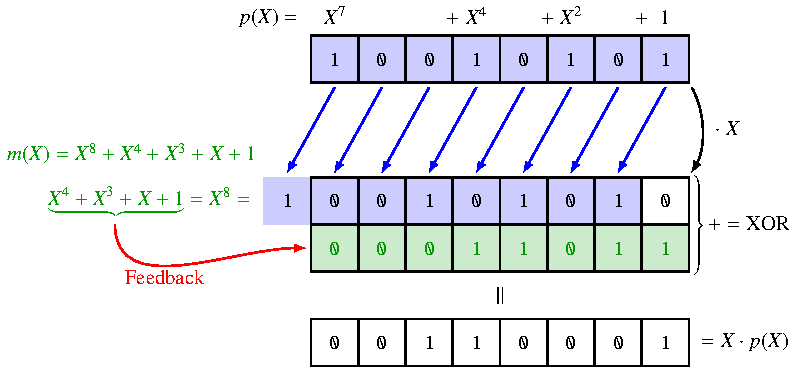
\includegraphics{chapters/90-crypto/images/schieberegister.pdf}
\caption{Implementation der Multiplikation mit $X$ in einem 
endlichen Körper $\mathbb{F}_{2^l}$ mit dem Minimalpolynom
$m(X) = X^8+X^4+X^3+X^+1$ als Feedback-Schieberegister.
\label{buch:crypto:fig:schieberegister}}
\end{figure}

\subsection{Rechenoperationen in $\mathbb{F}_{2^l}$
\label{buch:subsection:rechenoperatione-in-f2l}}
Von besonderem praktischem Interesse sind die endlichen Körper
$\mathbb{F}_{2^l}$.
Die arithmetischen Operationen in diesen Körpern lassen sich besonders
effizient in Hardware realisieren.

\begin{figure}
\centering
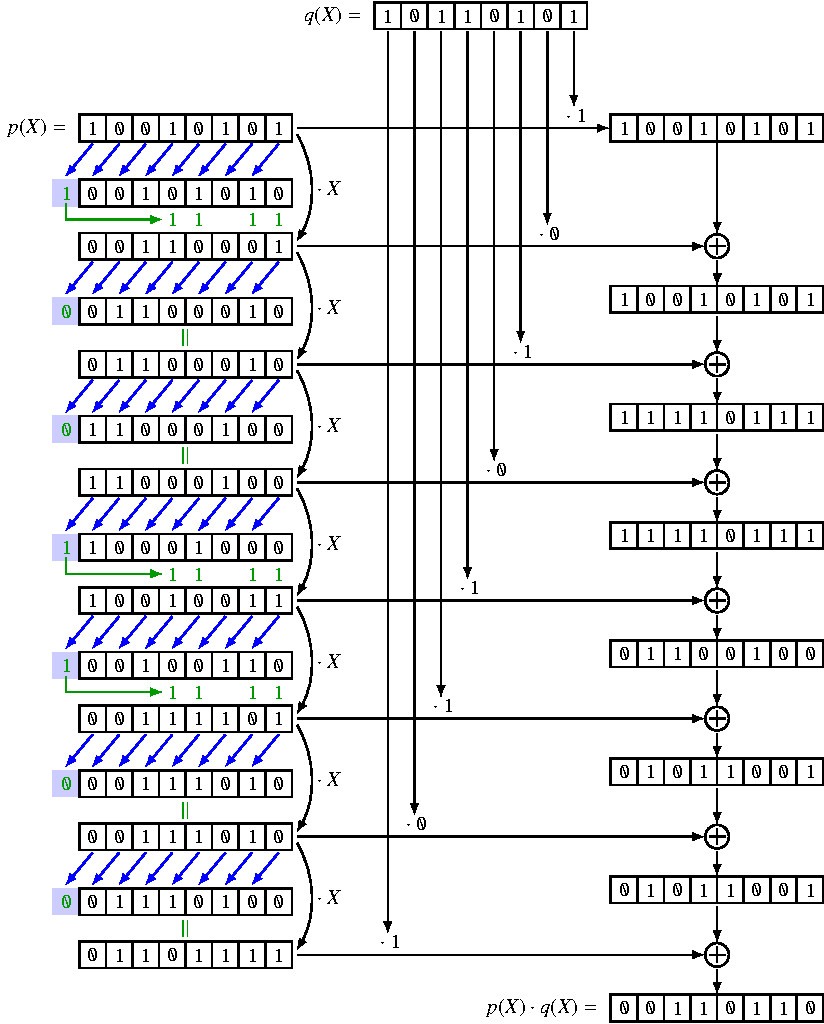
\includegraphics[width=\textwidth]{chapters/90-crypto/images/multiplikation.pdf}
\caption{Multiplikation zweier Elemente von $\mathbb{F}_{2^l}$.
Mit Hilfe des Schieberegisters am linken Rand werden die Produkte 
$X\cdot p(X)$, $X^2\cdot p(X),\dots,X^7\cdot p(X)$ nach der in
Abbildung~\ref{buch:crypto:fig:schieberegister} dargestellten
Methode berechnet.
Am rechten Rand werden diejenigen $X^k\cdot p(X)$ aufaddiert,
für die der $X^k$-Koeffizient von $q(X)$ von $0$ verschieden ist.
\label{buch:crypto:fig:multiplikation}}
\end{figure}

\subsubsection{Zahldarstellung}
Ein endlicher Körper $\mathbb{F}_{2^l}$ ist definiert durch ein
irreduzibles Polynom in $\mathbb{F}_2[X]$ vom Grad $2^l$ 
\[
m(X)
=
X^l + m_{l-1}X^{l-1} + m_{l-2}X^{l-2} + \dots + m_2X^2 + m_1X + m_0
\]
gegeben.
Ein Element in $\mathbb{F}_2[X]/(m)$ kann
durch ein Polynom vom Grad $l-1$
dargestellt werden, also durch
\[
a = a_{l-1}X^{l-1} + a_{l-2}X^{l-2} +\dots + a_2X^2 + a_1X + a_0.
\]
In einer Maschine kann ein Elemente von $\mathbb{F}_2[X]/(m)$
also als eine Bitfolge der Länge $l$
dargestellt werden.


\subsubsection{Addition}
Die Addition in $\mathbb{F}_2$ ist in Hardware besonders leicht zu
realisieren.
Die Addition ist die XOR-Operation, die Multiplikation ist die UND-Verknüfung.
Ausserdem stimmen in $\mathbb{F}_2$ Addition und Subtraktion überein.

Die Addition zweier Polynome erfolgt komponentenweise.
Die Addition von zwei Elemente von $\mathbb{F}_{2^l}$ kann also
durch die bitweise XOR-Verknüpfung der Darstellungen der Summanden 
erfolgen.
Diese Operation ist in einem einzigen Maschinenzyklus realisierbar.
Die Subtraktion, die für die Reduktionsoperation modulo $m(X)$ nötig
ist, ist mit der Addition identisch.


\subsubsection{Multiplikation}
Die Multiplikation zweier Polynome benötigt zunächst die Multiplikation
mit $X$, wodurch der Grad des Polynoms ansteigt und möglicherweise so
gross wird, dass eine Reduktionsoperation modulo $m(X)$ nötig wird.
Die Reduktion wird immer dann nötig, wenn der Koeffizient von $X^l$
nicht $0$ ist.
Der Koeffizient kann dann zum Verschwinden gebracht werden, indem
$m(X)$ addiert wird.

In Abbildung~\ref{buch:crypto:fig:schieberegister} wird gezeigt,
wie die Reduktion erfolgt, wenn die Multiplikation mit $X$, also der
Shift nach links, einen Überlauf ergibt.
Das Minimalpolynom $m(X)=X^8+X^4+X^3+X+1$ bedeutet, dass in $\mathbb{F}_{2^l}$
$X^8=X^4+X^3+X+1$ gilt, so dass man das Überlaufbit durch 
$X^4+X^3+X+1$ ersetzen und addieren kann.

Ein Produkt $p(X)\cdot q(X)$, wobei $p(X)$ und
$q(X)$ Repräsentaten von Elementen $\mathbb{F}_{2^l}$ sind, kann jetzt
wie folgt berechnet werden.
Mit einem Schieberegister werden die Vielfachen $X^k\cdot p(X)$ 
für $k=0,\dots,l-1$ berechnet.
Diejenigen Vielfachen, für die der Koeffizient von $X^k$ in $q(X)$
von $0$ verschieden ist werden aufsummiert und ergeben das Produkt.
Der Prozess in Abbildung~\ref{buch:crypto:fig:multiplikation}
dargestellt.




